\documentclass[a4,11pt,oneside]{article}
%\documentclass[a4,12pt]{practica}

\usepackage[english]{babel}
\usepackage{epsfig}
\usepackage{amssymb,listings,color,textcomp,marvosym,flafter,longtable,subfigure,amsfonts,rotating}
\usepackage[sumlimits]{amsmath}
\usepackage{verbatim}
\usepackage{latexsym}
\usepackage{multirow}
\usepackage{array,pstricks,listings}
\usepackage[a4paper,verbose, centering,reversemp]{geometry}
\usepackage[latin1]{inputenc} 
\usepackage{fancyhdr}
\usepackage{hhline}     % generates nicer table lines (without missing pixels) + more flexible
\usepackage[times]{quotchap} 
\usepackage[font={small},labelfont={bf},center]{caption}
% this package used to produce a different style of page numbering
%\usepackage{chappg}  
\usepackage{times}  
\usepackage{wrapfig}
\usepackage{floatflt}
% this package is used for colored text
\usepackage{xcolor}
% this package is used for intelligent spaces
\usepackage{xspace}
%\input{macros.tex}
\usepackage[calcwidth,newparttoc]{titlesec}
% use the titletoc package to change the toc
\usepackage{titletoc}
% this package is the natural frontend for pgf (a package for creating graphics in an inline manner).
\usepackage[round]{natbib}
\definecolor{chaptergray}{rgb}{0.85,0.85,0.85}
%\textwidth=15.5cm
%\textheight=23cm
\usepackage{enumerate}
\usepackage{pstricks,pstcol,pst-text,pst-node,pst-tree}
\usepackage{verbatim}
\usepackage[vlined,ruled,nederlands]{algorithm2e}
\usepackage{graphicx}
\usepackage{tabularx}
\usepackage{latexcad}
\usepackage{soul}
\usepackage{hyperref}
\usepackage{epstopdf}
\usepackage[framemethod=TikZ]{mdframed}
%\hypersetup{colorlinks=false}
\definecolor{silver}{rgb}{0.95,0.95,0.95}
\definecolor{chaptergray}{rgb}{0.95,0.95,0.95}
\font\sixly=lasy6 % does not re-load if already loaded, so no memory problem.

\usepackage{lmodern}
\usepackage[T1]{fontenc}

\mdfdefinestyle{warning}{%
    linecolor=white,
    align=center,
    roundcorner=3pt,
    innertopmargin=6pt,
    innerbottommargin=5pt,
    innerrightmargin=10pt,
    innerleftmargin=10pt,
    backgroundcolor=black!12,
    skipabove=0.4\baselineskip
}

%\input{macros.tex}

%\textwidth=15.5cm
%\textheight=23cm

\parskip=\medskipamount
%\parindent=0pt
\setcounter{secnumdepth}{3}
\newtheorem{mf}{MATLAB functie}[section]
\newtheorem{vb}{Voorbeeld}[section]

\newtheorem{voorbeelden}{Voorbeelden}[section]
\newtheorem{vraag}{Vraag}[section]
\newtheorem{opdracht}{Opdracht}[section]
\newtheorem{opdrachtE}{Assignment}[section]


\def\bea{\begin{eqnarray}}
\def\eea{\end{eqnarray}}
\def\beas{\begin{eqnarray*}}
\def\eeas{\end{eqnarray*}}

\def\pr{\mbox{Pr}}

\newtheorem{oefening}{Oefening}[section]
%\renewcommand\chaptername{Practicum}

\renewcommand{\algorithmcfname}{Algoritme}
%%%%%%%%%%%%%%%%%%%%%%%%%%%%%%%%%%%%%%%%%%%%%%%%%%%%%%%%%%%%%%%%%%%%%%
% document: page_layout_definition.tex
%
% last modified: $Id: page_layout_definition.tex,v 1.1 2005/11/18 11:49:23 bvolckae Exp $
%
% author: Filip De Turck, Stefaan Vanhastel, Bart Duysburgh, Brecht Vermeulen, Bruno Volckaert, Steven Van den Berghe
%%%%%%%%%%%%%%%%%%%%%%%%%%%%%%%%%%%%%%%%%%%%%%%%%%%%%%%%%%%%%%%%%%%%%%

%%%%%%%%%%%%%%%%%%%%%%%%%%%%%%%%%%%%%%%%%%%%%%%%%%%%%%%%%%%%%%%%%%%%%%

% basic dimensions when printing the small page %
% and by using the geometry package             %

% settings Filip en Stefaan
%\geometry{bottom=4.0cm,rmargin=4.25cm,body={12.5cm,19.5cm}} % 10pt op a4
%\geometry{marginpar=0.0cm,marginparsep=0.0cm,twosideshift=0.0cm}

% new settings (according book pim which was approved by the promotors) by Bart Duysburgh
%\geometry{bottom=5.34cm,rmargin=4.5cm,body={11.5cm,18.92cm}} % 10pt op a4
%\geometry{marginpar=0.0cm,marginparsep=0.0cm,twosideshift=0.0cm}
%body={16.5cm,24cm}
\geometry{bottom=2.5cm,rmargin=2.25cm,lmargin=2.5cm,top=2.6cm} % 10pt op a4
%\geometry{bottom=5.34cm,rmargin=4.5cm,body={11.5cm,18.92cm}} % 10pt op a4
\geometry{marginpar=2.5cm,marginparsep=0cm}

%\geometry{bottom=2.15cm,rmargin=2.5cm,body={14.14125cm,23.6cm}} % 12pt op a4

%\renewcommand{\headwidth}{17cm}                % Resetten van al de fancy settings.%
%\renewcommand{\headrulewidth}{0.4pt}      % Zet dit op 0.4pt voor een mooie lijn. geen lijn: 0pt
%\textwidth=15.5cm
%\textheight=23cm
%%%%%%%%%%%%%%%%%%%%%%%%%%%%%%%%%%%%%%%%
%\topmargin=0cm
%\headsep=.7cm
\setlength{\textwidth}{16.5cm}
%\setlength{\textheight}{24cm}
%\setlength{\topmargin}{0.0cm}
%\setlength{\oddsidemargin}{0.7cm}
%\setlength{\evensidemargin}{0.7cm}
%\setlength{\marginparwidth}{0pt}
%\setlength{\marginparsep}{0pt}


%%%%%%%%%%%%%%%%%%%%%%%%%%%%%%%%%%%%%%%

%\renewcommand{\topfraction}{0.8}

%%%%%%%%%%%%%%%%%%%%%%%%%%%%%%%%%%%%%%%

%%%%%%%%%%%%%%%%%%%%%%%%%%%%%%%%%%%%%%
%% change for subfigure
\renewcommand{\subfigcapskip}{0pt}
%%%%%%%%%%%%%%%%%%%%%%%%%%%%%%%%%%%%%%

%%%%%%%%%%%%%%%%%%%%%%%%%%%%%%%%%%%%%%%
% headings %

\fancypagestyle{plain}{
\fancyhf{}
\renewcommand{\headrulewidth}{0pt}
\renewcommand{\footrulewidth}{0pt}}

\pagestyle{fancy}
\fancyhf{} %clear all header and footer fields
%\addtolength{\headwidth}{\marginparsep}
%\addtolength{\headwidth}{\marginparwidth}

\renewcommand{\chaptermark}[1]{\markboth{\chaptername\ \thechapter. \ #1}{}}

%\renewcommand{\chaptermark}[1]{\markboth{#1}{}}
%\renewcommand{\sectionmark}[1]{\markright{\thesection\ #1}}

%\newcommand\fdtsvrightmarktmp{{\scshape\small Chapter }}
%\newcommand\fdtsvrightmark{{\scshape\small{Acknowledgment}}}
%\newcommand\fdtsvleftmark{{\scshape\small{Dankwoord}}}

%\newcommand\oddpageleftmark{}
%\newcommand\evenpagerightmark{}

%\fancyhead[LE,RO]{\itshape\bfseries\small\thepage}
%\fancyhead[HL]{\itshape\bfseries\small\leftmark}
%\fancyhead[RE]{\itshape\bfseries\small\rightmark}
%\fancyfoot[FC]{\bfseries\small\thepage}
%\fancyhead[LO]{\oddpageleftmark}
%\fancyhead[RE]{\evenpagerightmark}
%\fancyhead[HL]{\nouppercase{\leftmark}}
%\fancyfoot[C]{\itshape\bfseries\footnotesize \chaptername\ \thechapter}

%%%%%%%%%%%%%%%%%%%%%%%%%%%%%%%%%%%%%%%%%%%%%%%%%%%%


%%%%%%%%%%%%%%%%%%%%%%%%%%%%%%%%%%%%%%%%%%%%%%%%%%%%
% depth of numbering and depth of table of contents %

\setcounter{tocdepth}{3} % titels tot en met niveau subsubsection worden in table of contents opgenomen
\setcounter{secnumdepth}{3} % tot en met niveau subsubsection wordt er genummerd
%%%%%%%%%%%%%%%%%%%%%%%%%%%%%%%%%%%%%%%%%%%%%%%%%%%



%%%%%%%%%%%%%%%%%%%%%%%%%%%%%%%%%%%%%%%%%%%%%%%%%%%
%%%%% Definition for Big letter at the beginning of a paragraph %%
\def\PARstart#1#2{\begingroup\def\par{\endgraf\endgroup\lineskiplimit=0pt}
    \setbox2=\hbox{\uppercase{#2} }\newdimen\tmpht \tmpht \ht2
    \advance\tmpht by \baselineskip\font\hhuge=cmr10 at \tmpht
    \setbox1=\hbox{{\hhuge #1}}
    \count7=\tmpht \count8=\ht1\divide\count8 by 1000 \divide\count7 by\count8
    \tmpht=.001\tmpht\multiply\tmpht by \count7\font\hhuge=cmr10 at \tmpht
    \setbox1=\hbox{{\hhuge #1}} \noindent \hangindent1.05\wd1
    \hangafter=-2 {\hskip-\hangindent \lower1\ht1\hbox{\raise1.0\ht2\copy1}%
    \kern-0\wd1}\copy2\lineskiplimit=-1000pt}
%%%%%%%%%%%%%%%%%%%%%%%%%%%%%%%%%%%%


%%%%%%%%%%%%%%%%%%%%%%%%%%%%%%%%%%%%%%%%%%%%%%%%%%%%
%%% Nog een paar andere zaken  %%%%
%% om een cross-ref naar een voetnoot te kunnen maken definier ik \usefn %%
%\newcommand{\usefn}[1]{\mbox{\textsuperscript{\normalfont#1}}}
%
%\setlength{\captionindent}{1cm}
%\renewcommand{\captionfont}{\small \itshape \mdseries \rmfamily}
%\renewcommand{\subcapsize}{\footnotesize \itshape \mdseries \rmfamily}
%
%\AtBeginDocument{%
%%   \renewcommand{\figurename}{Fig.}%
%%   \renewcommand{\tablename}{TABLE}%
%   \renewcommand{\tablename}{Table}
%   \renewcommand{\bibname}{References}%
%}

%%%%%%%%%%%%%%%%%%%%%%%%%%%%%%%%%%%%%%%%%%%%%%%%%%%


\renewcommand{\baselinestretch}{1.2}
% space between two paragraphs should be larger than between two lines of text
\newcommand{\npar} {\par \vspace{2.3ex plus 0.3ex minus 0.3ex}} 
% no indentations
\setlength{\parindent}{0cm}
% makes all pages the height of the text on that page, and no extra vertical space is added
\raggedbottom
\renewcommand\chaptertitlename{PC-lab}


% define part label
\titleformat{\part}[display]{\flushright\bfseries\vspace{-10cm}} 
{\usefont{OT1}{pag}{b}{n}\fontsize{50}{54}\selectfont{PART~\thepart}} {0pt} {\vspace{0.5cm}\huge\usefont{OT1}{pag}{m}{n}\fontsize{25}{30}\selectfont\uppercase} [\thispagestyle{empty}\pagecolor{chaptergray}]
% define chapter label
\titleformat{\chapter}[display]{\flushright\vspace{-3cm}\pagecolor{white}}
{\usefont{OT1}{pag}{b}{n}\fontsize{34}{34}\selectfont {\chaptertitlename\quad\thechapter}}{10pt}{\usefont{OT1}{pag}{m}{n}\fontsize{22}{24}\selectfont}[{\thispagestyle{empty}\vspace{3cm}}]
% define section label
\titleformat{\section}[hang]{}
{\usefont{OT1}{pag}{b}{n}\fontsize{14}{16}\selectfont\thesection}{16pt}{\usefont{OT1}{pag}{b}{n}\fontsize{14}{16}\selectfont}[{}\vspace{0.25cm}]

\titleformat{\subsection}[hang]{}
{\usefont{OT1}{pag}{b}{n}\selectfont\thesubsection}{13pt}{\usefont{OT1}{pag}{b}{n}\selectfont}[{}\vspace{0.25cm}]
% define subsubsection label
\titleformat{\subsubsection}[hang]{\sffamily}
{\usefont{OT1}{pag}{m}{n}\fontsize{11}{12}\selectfont\thesubsubsection}{13pt}{\usefont{OT1}{pag}{m}{n}\fontsize{11}{12}\selectfont}[{}\vspace{0.05cm}]
% define paragraph label
\titleformat{\paragraph}[runin]{\sffamily}
{\usefont{OT1}{pag}{b}{n}\selectfont\theparagraph}{}{}[{}]

% define the headers and the footers
\renewcommand{\chaptermark}[1]%
 {\markboth{ \MakeUppercase{CHAPTER~\thechapter \mdseries{~~~#1}}}{}}
\renewcommand{\sectionmark}[1]%
 {\markright{\fontsize{10}{12} \selectfont\MakeUppercase{\thepart.\thesection \mdseries{~~~#1}}}}
\renewcommand{\headrulewidth}{0.15pt}
\renewcommand{\footrulewidth}{0pt}
\newcommand{\helv}{%
\fontfamily{phv}\fontseries{b}\fontsize{8}{10}\selectfont}
\fancyhf{}
\fancyhf[HR]{\helv \fontsize{10}{12} \selectfont \thepage}
\fancyhf[HL]{\helv \fontsize{10}{12} \selectfont \rightmark}
%\fancyhf[HL]{\helv \rightmark}
%\fancyhead[RE]{\helv \rightmark}


%\texttt{}
\hyphenation{bij-ge-volg ge-wij-zigd toe-pas-sing toe-pas-sing-en
lid-maat-schaps-func-ties ver-ge-lijk-ing-en va-ria-be-le
pa-ra-me-ter-s pa-ra-me-ter in-gangs-var-ia-be-le
uit-gangs-var-ia-be-le glo-ba-le sym-bo-li-sche be-schik-king
ver-wer-ven zoek-me-tho-den pro-ba-bi-li-teit ge-ne-ra-tie
ver-dui-de-lij-ken de-co-de-ring af-wij-king-en drie-hoe-ki-ge
tra-pe-zo clus-ter-al-go-rit-mes uit-ein-de-lijke tracht fi-gu-ren ge-lijk-aardig mo-ge-lijke ge-lijk-aardige op-ti-ma-li-sa-tie-pro-ble-men pro-bleem-spe-ci-fie-ke}

\lstset{language=R,commentstyle=, framexleftmargin=5mm,belowcaptionskip=5mm, frame=single,basicstyle={\ttfamily\small}, stringstyle=\small,commentstyle=\textcolor[rgb]{0.53,0.53,0.53}, backgroundcolor=\color[rgb]{0.93,0.93,0.93},showspaces=false,framexleftmargin=-2pt,showstringspaces=false,upquote=true}

\begin{document}
%\frontmatter
\renewcommand{\algorithmcfname}{Algorithm}
\pagestyle{empty}


\begin{titlepage}
	\begin{center}
		%{\rugfnt A}\\[.3cm]
		{\Large\bf GHENT UNIVERSITY}\\[.5cm]
		{\Large Faculty of Bioscience Engineering}\\[.5cm]
		{\Large Department of Mathematical Modelling, Statistics and Bioinformatics}\\[.5cm]
		\hrule{\ }\\[.4cm]
	
		\vspace{3cm}
\begin{mdframed}[style=warning]
		\vspace{1cm}
\centering
		{{\huge \bf Machine Learning for Image Processing}}\\[1cm]
		{\LARGE Predictive Modelling - Project 1}
		\vspace{1cm}
\end{mdframed}
		\vspace{0.5cm}


	\end{center}
	
	\begin{center}
		{
		\large \bf ir. Michael Ghijs\\[.2cm]
		\large \bf ir. Jim Clauwaert\\[.2cm]
		\large \bf ir. Marlies Volckaert\\[.2cm]
%		\\[.1cm]
		}%\\
		\vspace{1cm}
		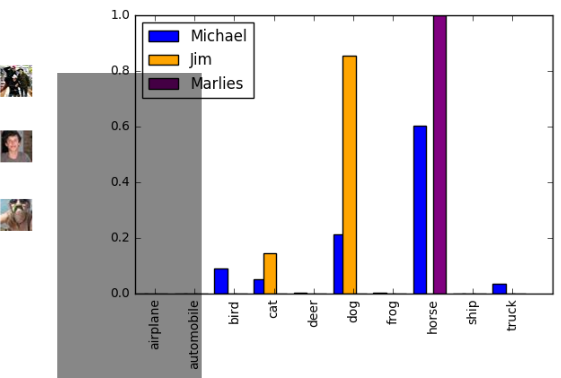
\includegraphics[width=0.6\textwidth]{../figures/cifar_alles}


		
		\vspace{1cm}
%		Master in Bioscience Engineering\hfill
		Academic year 2016--2017\\[.3cm]
		\hrule \vspace{.3cm}
%		\noindent {\tt http://www.kermit.ugent.be}
		% \noindent {\tt http://biomath.UGent.be/\~{ }kcmaes}
	\end{center}
\end{titlepage}





%%%  --> BEGIN OLD frontpage

%\begin{titlepage}
%\begin{center}
%%{\rugfnt A}\\[.3cm]
%{\Large\bf GHENT UNIVERSITY}\\[.5cm]
%{\large Faculty of Bioscience engineering}\\[.4cm]
%\hrule{\ }\\[.4cm]
%{\large Department of Mathematical Modeling, Statistics and Bioinformatics}
%
%\vspace{3cm} {\Huge \bf Machine Learning:\\[1cm]
%PC-labs}
%\end{center}
%
%\begin{center}
%\vspace{2cm} {\Large \bf Prof.\ Dr.\ Bernard DE BAETS\\[.1cm]
%Dr. Willem WAEGEMAN\\[.25cm]
%Ir. Jan VERWAEREN}
%\vspace{2cm}
%\begin{center}
%\includegraphics[width=3.5cm]{figures/Kermit.eps}
%\end{center}
%\vfill
%Course notes for\\[.3cm]
%``Machine Learning''\\[.3cm]
%Master in Bioscience engineering\\[.3cm]
%Academic year 2012--2013\\[.3cm]
%\hrule
%\vspace{.3cm}
%
%\noindent {\small\tt http://www.kermit.ugent.be}
%\end{center}
%%\end{document}
%\newpage
%~ 
%\end{titlepage}

%%%  --> END OLD frontpage






%\newpage
%\pagestyle{empty}
%~
%\newpage
%\setcounter{page}{1}
%\pagestyle{fancy}
%\tableofcontents
%\newpage
%\thispagestyle{empty}
~
%\mainmatter
%\setcounter{page}{-1}
%\part[Introduction To Machine Learning]{Introduction To\\ Machine Learning}

%\pagestyle{empty}
%\newpage
%~
%\newpage
%\pagestyle{fancy}
%\setcounter{page}{1}

%\parindent=0cm
%\setcounter{chapter}{7}
%\documentclass{article}
%\usepackage{graphicx}
%\usepackage{tabularx}
%\usepackage [dutch] {babel}
%\usepackage[vlined,ruled,algo2e]{algorithm2e}

\newcommand{\xvect}{\mathbf{x}} 
%\chapter[Scientific programming for Machine Learning]{Scientific programming for\\ Machine Learning}
%\begin{document}
%\chapter{\emph{Hill Climbing} en \emph{Simulated Annealing}}\label{pract: HC}
\section{From cable transmission to far beyond: \\ applications and evolution of image processing \label{sec:evolution}}
Early digital image processing began in the early 1920s with the Bartlane cable picture transmission system that was used to transmit newspaper images across the Atlantic (Figure~\ref{fig:bartlane}). The images were coded and sent by telegraph. It took about three hours to send an image and the first systems supported only five grey levels. Along with the first satellite images in the beginning of the 1960s, image processing further emerged. Although computers were slow at the time and their processing capacity very limited, image processing was used for weather forecasting, military purposes, land use detection etc. 
\begin{wrapfigure}{R}{0.6\textwidth}
	\centering
	\includegraphics[width=0.5\textwidth]{../figures/Bartlane}
	\caption{Code used by the Bartlane transmitter to transport newspaper images.
		\label{fig:bartlane}}
\end{wrapfigure}

As the computers evolved, so did digital image processing and algorithms became more and more complex: today, automated image recognition is omnipresent. Think about Google images, criminal detection, fingerprint scans at the airports, smart radars, detection of cancer cells etc. 


Computer vision, or machine vision, means the use of digital processing and intelligent algorithms to interpret meaning from images or video. Machine vision definitely is a hot item: currently self-driven cars and buses are in full development and the first prototypes are being tested which make use of 3D-real time computer vision. 

%\begin{figure}[h]
%	\centering
%	\includegraphics[width=0.5\textwidth]{../figures/Mesta-Fusion}
%	\label{fig:flitspaal}
%	\caption{The Mesta Fusion traffic radar is coming to our roads and is already operational in some European countries. It uses machine vision technologies to track 32 cars at a time, for license plate recognition among others.}
%\end{figure}



\begin{wrapfigure}{l}{0.6\textwidth}
	\centering
	\includegraphics[width=0.5\textwidth]{../figures/Mesta-Fusion}
	\caption{The Mesta Fusion traffic radar is coming to our roads and is already operational in some European countries. It uses machine vision technologies to track 32 cars at a time, for license plate recognition among others. \label{fig:flitspaal}}
\end{wrapfigure}
Today a major transformation is underway. Due to the emergence of very powerful, low-cost, and energy-efficient processors, it has become possible to incorporate practical computer vision capabilities into embedded systems, mobile devices, PCs, and the cloud. Over the next few years, there will be a rapid proliferation of embedded vision technology into many kinds of systems. Take `Project Tango' from Google as an example: it uses (small) smartphone cameras to picture the 3D-structure of the space in which a person is situated. 

Just imagine this technology in real-time games!



\section{From human vision to computer vision: principles and mechanisms \label{sec:mechanisms}}
When a 3-year child looks at an image, it can already detect what it sees: an airplane taking off, a cat sitting on a couch, a tree in a park, etc. That child is already an expert in making sense to what it sees. Our most advanced technological systems still struggle with this task.
The human eye is a sensor that catches light on the retina, the optic nerve transports the impulses to the brains and there the magic happens: sophisticated neural networks analyze the images and give meaning to it. Vision begins at the eyes, but it truly takes place in the brains. 
Computer vision is based on the same principles as human vision. Cameras register the incoming light as digital numbers in a 2D (or 3D) array. Besides the intensity of the incoming light, pixels do not have a meaning, they do not say what is in the picture. In order to understand a picture, a computer needs to apply the entire Image Processing Chain, see Figure~\ref{fig:imProChain}:

\begin{figure}[h!]
	\centering
	\includegraphics[width=\textwidth]{../figures/imageProcessingChain}
	\caption{Classical image processing chain.  \cite{Egmont-Petersen2002} 
		\label{fig:imProChain}}
\end{figure}

\begin{enumerate}
	\item \textbf{Preprocessing}:
	Images can contain a lot of noise and could therefore difficult to interpret. Think for example of Rayleigh scattering in satellite images which result in a very low contrast, or photographs that look blurry because they were taking while moving. Preprocessing consists of operations that modify the original image in order to make it more interpretable: e.g. noise reduction and contrast enhancement.
	
	
	\item \textbf{Data reduction}:
Hyperspectral satellites process incoming light at more than thousand different spectral bands. The information coming from this images is enormous and not all information is equally useful. Only the bands which carry the most information for a specific application are selected. If we take a look to a single image, features (entropy, contrast, heterogeneity etc.)  can be extracted by means of moving windows. The number of features extracted is generally smaller than the number of pixels in the input window. 

\item \textbf{Segmentation}:
The partitioning of the image into regions with similar characteristics (spectral, textural features). 

\item \textbf{Object detection and recognition}:
Once the image is divided into segments, these segments can be classified. The position, orientation and scale of objects (possibly consisting of multiple segments) can be determined. 

\item \textbf{Image understanding}:
Deriving high level knowledge, semantic data, from an image. E.g. there is a cat on the table (and the cat is hungry trying to steal pork ribs).

\end{enumerate}

\section{Copying the brain: Convolutional Neural Networks \label{sec:cnn}}
\textit{Neural networks} are a computational approach inspired by the structure of the brain, as the resulting models are large collections of interconnected neurons, connecting inputs to a prediction (Figure~\ref{fig:ann}). They are used in various image processing applications, e.g. to optimise different steps in the image processing chain. \textit{Convolutional neural networks} are a more recent strategy in artificial intelligence, using neural networks to copy the abilities of a three-year-old child in image recognition.
\begin{figure}[h!]
	\centering
	\includegraphics[width=\textwidth]{../figures/ann_struct}
	\caption{Neural network.
		\label{fig:ann}}
\end{figure}

\subsection{The basics: Neural networks \label{subsec:neural}}
Neural networks process a number of inputs with a set of artificial \textit{neurons} in order to generate its model output, i.e. a prediction. These neurons individually can take in multiple inputs and process them in two steps to formulate an output: aggregation of the inputs and consecutively linking them to the output with an activation function. The output is a certain value representing the (amount of) activation of the neuron. 


In the \textit{aggregation step}, \textit{weights} ${w}$ are given to the different inputs of the neuron, indicating their influence on the neuron\textquoteright s output. The weights are multiplied with the input values and summed, calling for a \textit{threshold} or \textit{bias} ${b}$, to tell whether or not the aggregated value leads to activation of the neuron. If $\sum{{wx}} > {b}$, the neuron is activated, otherwise it is not; this can be seen as a step function between 0 and 1.


This would be the basic construction for the neuron, yet the step function can prove cumbersome for the training of the neural network. Therefore, the aggregated value and bias themselves are linked to the actual neuron output by an \textit{activation function} $f(a)$ (Equation~\ref{eq:actfun}). The commonly used activation functions are presented in Section~\ref{subsec:activation}. 

\begin{equation} \label{eq:actfun}
f(a) = f\left(\sum{{wx}} - {b}\right)
\end{equation}

The output of neurons can then be connected to other neurons. The structure of a neural network usually consists of layers of neurons, the first one processing the inputs and passing on their outputs to the second layer, while the last layer generates the prediction (see Figure~\ref{fig:ann}). This is detailed in Section~\ref{subsubsec:archi}.


\subsubsection{Commonly used activation functions \label{subsec:activation}}
A historically used function, attractive because of its similarity to the biological neuron, is the \textit{sigmoid function}, presented in Equation~\ref{eq:sig} (Figure~\ref{fig:actifun}, second from the left). It `squashes\textquoteright  a real input into the range between 0 and 1. Neural network applications have moved on from this function however. As the tails of the function have a very low slope - which is used in training the neural network (see section later on) -  the sigmoid function can cause that the neuron goes unnoticed during training. Next to this major drawback, a minor inconvenience of the sigmoid function is that the output is always positive, of which the consequences will be explained in Section~\ref{subsubsec:training}.
\begin{equation} \label{eq:sig}
f(a) = \frac{a}{1+e^{-a}}
\end{equation}

A similar activation function is \textit{Tanh}, Equation~\ref{eq:tanh} (Figure~\ref{fig:actifun}, middle), which has a similar shape as the sigmoid function and mitigates the aforementioned issue by squashing its input between -1 and 1, allowing for negative output values. 
\begin{equation} \label{eq:tanh}
f(a) = \frac{e^{a}-e^{-a}}{e^{a}+e^{-a}}
\end{equation}

Another function, the \textit{Rectified Linear Unit} or \textit{ReLU}, Equation~\ref{eq:relu} (Figure~\ref{fig:actifun}, second from the right), basically thresholds the input at 0. They were found to greatly accelerate training of the neural network \cite{Krizhevsky2012}, said to be due to its linear form. Compared to the first two activation functions, ReLUs are easy to implement and to compute. Despite their popularity, ReLUs have the major drawback that they can \textquoteleft die\textquoteright\   during training, which means that they do not activate on any datapoint anymore. This can occur in the case that a large gradient flows through the neuron, which could lead to the weights being updated in a way that no inputs can still activate the neuron. At high learning rates the risk of this \textquoteleft death\textquoteright\   is high and large part of the network can turn out to be deactivated.
\begin{equation} \label{eq:relu}
f(a) = \max(0, a)
\end{equation}

To accommodate for the ReLU \textquoteleft neuron death\textquoteright\   issue, \textit{Leaky ReLUs}, Equation~\ref{eq:leaky} (Figure~\ref{fig:actifun}, first from the right) have a small constant positive slope at levels below 0.
\begin{equation} \label{eq:leaky}
f(a) = \max(c\ast a, a) \ \ \mathrm{with}\ \  c\approx 0
\end{equation}

\begin{figure}[h]
	\includegraphics[width=\textwidth]{../figures/actiFunc}
	\caption{Output of some commonly used activation functions. \label{fig:actifun}}
\end{figure}
Last but not least is the \textit{softmax} function, Equation~\ref{eq:softmax}, which is distinct from the aforementioned activation functions because it relates the output of a single neuron to the outputs of all neurons in the layer. By dividing by the sum of all these outputs, the output of a single softmax neuron is always between 0 and 1, and the sum of all activations is 1. 

\begin{equation}\label{eq:softmax}
f(\mathbf{a})_i = \frac{e^{a_i}}{\sum_{j=1}^k e^{a_j}}
\end{equation}
%Finally, there are also activation functions that are out-of-the-box, such as the Maxout neuron. This activation function takes the maximum of the output of two different activation functions computed on the input. While this can solve issues related to the aforementioned functions, the amount of parameters in the model is increased.

\subsubsection{Network architecture \label{subsubsec:archi}}
Neural networks are usually built out of \textit{layers of neuron}s, in which a layer can be seen as a group of neurons where information can only be propagated to the next layer, thus without having connections between neurons in the same layer (visible in Figure~\ref{fig:ann}). These are \textit{feedforward neural networks}, yet other classes of neural networks also exist, such as recurrent neural networks, which do allow self loops on neurons.


%The \textit{size} of a neural network is usually expressed in the number of neurons or, even more commonly, as the number of parameters in the network. For example, the network in FIgure has this amount of parameters. Convolutional neural networks nowadays contain on orders of 100 million parameters and are usually made up of approximately 10 to 20 layers.
% % %%EXAMPLE

\subsubsection{Training a neural network \label{subsubsec:training}}
Training a neural network means optimising its parameter values so that its prediction $\mathbf{f}(\textbf{x})$ is as close to the real data $\textbf{y}$ as possible. The difference between the predicted and real values is represented by a \textit{loss function} $\mathcal{L}$. This function can take the form of a quadratic function, such as the SSE, yet this could result in a \textit{learning slowdown problem} due to the nature of the neurons. In a multi-class classification problem, which is common in image processing, taking for example the sigmoid neuron, one can see that in the tails of the output the slope is very low. Therefore, for these problems, a specific loss function has been developed, called \textit{cross-entropy} (Equation~\ref{eq:crossent}). 
\begin{equation} \label{eq:crossent}
\mathcal{L}_i(\mathbf{w}, \mathbf{b}) = -\sum_{i=1}^{n} y_i \log(f(\mathbf{x})_i)
\end{equation}
This loss function takes into account the structure of the activation function. Namely, when the cross-entropy loss function is derived to the network parameters, it is proven that this derivative is dependent on the difference between the neuron output and the real data. Ergo, the larger this difference, the faster the weights are changed to find a better optimum.


Other loss functions can still be applied in cases where these are feasible. Also, in the case of a softmax neuron layer, the learning slowdown problem is already intrinsically addressed.


For \textit{minimising} the loss function, the slope or \textit{gradient} of the loss function, in function of the model output, is the starting point. Following the gradient towards a minimum is therefore the mechanism in the most used optimisation algorithm for neural networks, namely \textit{gradient descent}. Another reason for its popularity though, is that the gradient can also be found for the loss function in function of the values of the model parameters. This technique is called \textit{backpropagation} and applies the chain rule of function derivatives. With this gradient, a set of optimal values for the parameters can immediately be explored for using gradient descent, a feature that allows for a much faster neural network training than by using other gradients.

\subsection{Convolutional neural networks \label{subsec:cnn}}

Convolutional neural networks (CNN) are neural networks with distinctive properties in the architecture that make them fit for, among others, image processing. A computer is only able to read an image as a set of pixels with different real values for certain features (e.g. RGB-values). A CNN will recognize higher-level features (see Section~\ref{sec:mechanisms}) based on these basic inputs.
\subsubsection{Network architecture \label{subsubsec:convarchi}}
\begin{wrapfigure}{R}{0.5\textwidth}
	\includegraphics[width=0.5\textwidth]{../figures/cnn_archi}
	\caption{Convolutional neural network architecture. Source: \url{http://cs231n.github.io/convolutional-networks/}\label{fig:cnnArchi}}
\end{wrapfigure}
Whereas in a regular neural network the neurons are organised in 2D-layers, these structures are complemented with a third dimension in CNNs (Figure~\ref{fig:cnnArchi}). The width and height of this structure could respectively represent the width and height of a detected area (of the image) in pixels. The depth then represents the amount of features that were read.

The convolution aspect of a CNN consists of each of the features being detected for a small piece of the image, e.g. a window of $3\times\time 3$ pixels. The CNN will slide this window over the entire image, producing a 2D activation map, i.e. the activation for every position of the window. The network will learn to recognize basic features in these windows, e.g. edges. Using the output of the activation map as input for another CNN, will allow this last CNN to detect higher-level features! For example, based on the edges, certain shapes could be derived. 

The concept of CNNs is illustrated by applying it to an image of a wild boar (Figure~\ref{fig:pyjama}). The image consist of a 2D-array of pixels with a certain gray-level intensity. The image is split into pieces and for each of these, $A$ will compute features. In fact, $A$ is a neural network. All neural networks get the same input pixel values and compute different features (contrast, entropy, homogeneity among others). If the piece contains e.g. a \textquoteleft pyjama\textquoteright\   (other word for a wild baby boar), this will result in a specific vertical texture: high frequency (repetition of very bright pixels, followed by very dark pixels). In the snow regions on the other hand, contrast will be very low.

\begin{figure}[h]
	\centering
	\includegraphics[width=0.6\textwidth]{../figures/pyjama2}
	\caption{Basic CNN applied to image of baby boar. \label{fig:pyjama}}
\end{figure}

The activation functions that are often used for interconnecting the networks are ReLUs (Equation~\ref{eq:relu}). Subsequently, to reduce data, convolutional layers are often interweaved with pooling layers. \textit{Maximum pooling} takes the maximum of features over a small block of input neurons. For a given patch of pixels the output of the maximum pooling step tells us if their is a high frequency, but not exactly where the high frequency is located. Maximum pooling has the benefit that higher layers can work on larger sections of data and that the output is made invariant to very small transformations of the data.

The output of the pooling layer is then used as input for \textit{fully connected convolution layer} ($F$) and fed into the final neural network that is able to predict whether or not wild boar babies are present in the image. This would often be in the form of a probability that the image is a boar or not. This is a binary classification problem. The output could also be in the form of probabilities that the picture contains a boar, a moose or another animal, resulting in a multi-class problem. One can see that a softmax activation function is suited for this kind of output of the fully connected layer. 
 

It is important to note that the entire classical image processing chain is integrated into this convolutional neural network. The separate steps are implicitly present at the different stages. Moreover, images are deliberately blurred to be used as input for these models so that the algorithm is capable of detecting objects regardless of any image artifacts. This is a major stumbling block: machine learning only works when you have -a lot of- data to train the model! 
\section{Image processing in practice}
As the (top layer of) the theory on CNNs is now covered, the remainder of the document deals with how image processing comes into practice, including our own take on applying and adapting CNN.
\subsection{Neural Network Libraries \label{sec:libraries}}
A variety of libraries are available for image analysis using neural networks. For Python, the programming language chosen to use in this report, multiple options exist. Tensorflow, an open source library released by Google Brain, can be considered the most popular choice at this time. Since its release in November 2015, the project has enjoyed over 11.394 commits from over 500 different contributors on GitHub \url{https://github.com/tensorflow/tensorflow} . The library is used across the majority of services offered by Google. The library uses Python for its API, while counting on the C++ programming language for under the hood calculations. 


TFlearn is a library built on top of TensorFLow to provide a higher-level API, offering the user more intuitive and easy-to-use functionality for the creation and implementation of neural networks. Although first released in late March 2016, it has received high popularity with contributions from over 60 developers \url{https://github.com/tflearn/tflearn}.

\subsection{Image datasets \label{subsec:imdata}}
The validation of deep neural networks for image processing techniques are highly partitioned into the specific function of the model and the type of data it is optimized for. As trained models are highly correlated to those parameters, their performance is dependent on the dataset it is validated with. A model can be created to recognize a single object for its input, but can also be engineered to recognize different objects from a scene, and partition it accordingly. Other models are trained to recognize and extract faces from moving pictures (video) or are specialized in the recognition of a single function. (e.g. reading the house number from street view pictures). 


As the quality of a model is highly dependent upon the function it performs, a variety of high quality datasets are used, upon which model optimization is continuously performed. Examples of used image datasets are MNIST, CIFAR10, CIFAR100 and The Street View House Numbers dataset (SVHN). The MNIST database is a collection 70.000 handwritten digits centered on a grayscale 28 by 28 pixel image.  It has long been the standard dataset for the comparison of methods for a wide range of machine learning techniques. A compendium listing high accuracy models over a broad range of machine learning techniques is featured on the MNIST website (\url{http://yann.lecun.com/exdb/mnist/}). Techniques include SVM, Non-Linear Classifier, K-Nearest Neighbors and Neural Networks. 

CIFAR10 and CIFAR100 are a collection of coloured (three layers) 32 by 32 pixel images featuring a centered object.  Both feature 60.000 images, where CIFAR10 features ten different labels and CIFAR-100 a hundred. The SVHN dataset furthermore features a set of 73.257 images of one or more digits featured in a 32 by 32 image. Unlike training on the MNIST dataset, models require the ability to extract and recognize multiple digits on one image. The documentation on new techniques adapted for training a model on one of these datasets with the resulting accuracy and error can be found here:   (\url{http://rodrigob.github.io/are_we_there_yet/build/classification_datasets_results.html}).


\subsection{Practical use-case \label{subsec:case}}
In this practical use-case we will aim to train a model to recognize humans. As no supercomputers were available for this work, tiny images are used to limit data processing requirements. For this, the CIFAR-100 dataset was used as a base and further enriched with images from humans. Only two possible predictions are executed by the model, being either \textquoteleft human\textquoteright  or \textquoteleft not human\textquoteright . This further limits the requirements of the processor, since highly accurate training is achieved in a faster and more simple way than training to recognize a high amount of labels. 
The CIFAR100 dataset has both coarse and fine labels. There are one hundred fine labels dividing the dataset. For every five fine labels, there is a superclass that encompasses all five classes: the coarse label. Specifically, CIFAR100 has  the coarse label \textquoteleft human\textquoteright  which consists of the five classes \textquoteleft baby\textquoteright , \textquoteleft boy\textquoteright , \textquoteleft girl\textquoteright , \textquoteleft man\textquoteright and \textquoteleft woman\textquoteright. After importing the required packages, we change the labels for human pictures to be class 1 and labels that are not human to be class 2.

Since our dataset contains mainly pictures of not humans, we wish to increase our pool of pictures of humans. For this, we enriched the CIFAR100 dataset with the Frames Labeled In Cinema (FLIC) (\url{http://bensapp.github.io/flic-dataset.html})  dataset and images from the WIDER FACE dataset (\url{http://mmlab.ie.cuhk.edu.hk/projects/WIDERFace/}). We changed all the labels for these datasets to \textquoteleft 1\textquoteright . An overview of all the used data is given in Table~\ref{tab:data}. Listing~\ref{fullCode} gives the complete code with annotation used for the use-case. 

\begin{table}[h]
	\centering
	\caption{Data used to train and test the model. \label{tab:data}}
	\begin{tabular}{l|llll}
		\textbf{() = \% human} & \textbf{CIFAR100} & \textbf{FLIC} & \textbf{LFW} & \textbf{Total} \\ \hline
		\textbf{Train}         & 50000 (5\%)                            & 3528 (100\%)                       & 11233 (100\%)                     & 64761 (26.65\%)                     \\ \cline{1-1}
		\textbf{Test}          & 10000 (5\%)                            & 1026 (100\%)                       & 2000 (100\%)                      & 13026 (27.00\%)                     \\ \cline{1-1}
		\textbf{Total}         & 60000 (5\%)                            & 4554 (100\%)                       & 13233 (100\%)                     & 77.787 (26.72\%)                    \\ \cline{1-1}
	\end{tabular}
\end{table}



After obtaining and processing our input data, the main function is executed. For this, we use the example function from TFLearn to create a model using CIFAR10 (\url{https://github.com/tflearn/tflearn/blob/master/examples/images/convnet_cifar10.py}). As our resources are limited, and our model is only meant to be used as a proof of concept, only 15 full iterations (epochs) over the whole dataset are done while executing the code.
\subsection{Gradient descent variants \label{subsec:gradient}}
Image recognition through the use of deep neural networks is still in its early phase as a study domain, where many new techniques are tried out on models to understand their interactions. Techniques in determining the optimal parameters are typically determined through the use of minimizing cross-entropy. Gradient descent, the determination of the gradient of  a specific set of parameters, can be used to achieve the goal of finding minima. Multiple techniques have been created that are identified through the way in which the gradient of a set of parameters is used to determine a new set of parameters. Where we first discussed ways to obtain a gradient, a short introduction is now given on different ways of using the obtained information.
\subsubsection{Momentum \label{subsubsec:momentum}}
Momentum helps to accelerate finding a minimum as it takes into account the gradient of the previous step. Doing this, it tries to dampen the oscillation of the different gradients. 
$$v_t = \gamma v_{t-1} + \eta \nabla_\theta J( \theta)$$
$$ \theta = \theta - v_t $$
Where $J( \theta)$ is the loss function with respect to the parameters $\theta$, $v_t$ the vector of signifying the change of the parameters at time step $t$ and  $\gamma$ the momentum term. The momentum term decides the importance of the gradient of the previous set of parameters.
\subsubsection{Nesterov accelerated gradient \label{subsubsec:nesterov}}
The Nesterov accelerated gradient (NAG) takes into account the possibility that the momentum algorithm can adjust the parameters too much, missing a minimum and possibly ending up with a parameter set that leads to a different minimum. Instead of predicting the gradient of the loss function for the current step of parameters, NAG takes the gradient of the set of parameters that has already been adjusted by the momentum of the previous iteration, as displayed in Figure~\ref{fig:nag}.

\begin{figure}[h!]
	\centering
	\includegraphics[width=0.6\textwidth]{../figures/nag}
	\caption{Depiction of the Nesterov accelerated gradient. Blue vector indicate the change of the set of the parameter of the momentum algorithm. The small vector represents the current gradient while the large vector signifies the updated accumulated gradient. The red vector indicates the gradient of the parameter set after adjustment by the accumulated gradient of the momentum (brown vector), resulting in an adjusted set of parameters (green vector).
		\label{fig:nag}}
\end{figure}

$$v_t = \gamma v_{t-1} + \eta \nabla_\theta J( \theta - \gamma v_{t-1})$$
$$ \theta = \theta - v_t $$

\subsubsection{Adagrad, Adadelta and Adam \label{subsubsec:aaa}}
Adagrad, Adadelta and Adam are a set of techniques implemented to adapt the learning rate to the frequency for which a parameter is updated. Specifically, the learning rate of more frequent parameters is dampened over time, while parameters linked to sparse data are not affected. Adagrad was a first implementation of this principle for which the learning rate of the respective parameters diminishes according to the sum of squares of the gradients with respect to $\theta{i}$. Adadelta is an adjustment to  Adagrad, dealing with an monotonically decreasing learning rate, using a decaying sum of squares to prevent the parameter to become too big. Adam, the latest and most used adjustment of the group keeps track of both the average of past gradients and squared gradients, having proven to be an even better technique in reaching the minimum efficiently.

\subsection{Results}

Figure \ref{fig:results} gives the output of TensorFlow after the training of the model is done. An accuracy of ca. 96\% is given. Alhough this is a high accuracy, and the model is very good at what it does, it demands considerations at the question: "What does the model do ?" or "What is the model good at?". Table \ref{tab:conf} gives a confusion matrix of predictions of the model for the test set. It can be noticed that the fa

However, when we try to predict images for the CIFAR10 dataset, which contains pictures of a class of objects or animals that have not been fed into the model, the model predicts that around half of the CIFAR10 database is human. Indeed, the trained model is great at separating humans from any of the entities considered in the CIFAR100 dataset, but when confronted with objects it has not seen before, it fails badly. Thus, we can say that the model is not trained to recognize humans from no humans, but it is trained to separate humans from the classes present in the CIFAR100 dataset. As it often goes with neural networks, to create a model able to reach our goal, (a lot) more data is needed.

\begin{figure}[h!]
	\centering
	\includegraphics[width=0.9\textwidth]{../figures/result.png}
	\caption{Output given by TensorFlow after training the model. Listed are total epochs, iterations, loss and accuracy scores.
		\label{fig:results}}
\end{figure}
\begin{table}[h]
	\centering
	\caption{Confusion matrix. \label{tab:conf}}
	\begin{tabular}{l|llll}
		& \textbf{Predicted no human} & \textbf{Predicted human} \\ \hline
		\textbf{True no human}         &    9485                        & 447   \\ 
		\textbf{True human}          & 15                         & 2378     \\
	\end{tabular}
\end{table}




\section{Appendix}
\lstset{upquote=true}
\begin{lstlisting}[caption= Code used to import and train the model classifying humans from no humnans, label=fullCode, basicstyle=\ttfamily\tiny, language=Python, stringstyle=\ttfamily,]

# Import packages
import tensorflow as tf
import tflearn
import numpy as np
from CIFAR100 import get_cifar100

# Import data into numpy array
datapath =  "/home/data/jclauw/workspace/tensorflow/CIFAR100/cifar-100-python/" 
tr_data100, tr_clabels100, tr_flabels100, te_data100, te_clabels100, 
	te_flabels100, clabel_names100, flabel_names100 = get_cifar100(datapath)  

# Reshape numpy array
tr_cifar100 = tr_data100.reshape(50000,32,32,3)/255
te_cifar100 = te_data100.reshape(10000,32,32,3)/255

# Change labels
te_labels = np.array([0 if u!= 14 else 1 for u in te_clabels100])
tr_labels = np.array([0 if u!= 14 else 1 for u in tr_clabels100])

# Import data from LFW and FLIC database
XtrainLFW, YtrainLFW = tflearn.data_utils.image_dirs_to_samples(directory='~/', 
		resize=(32,32), filetypes=['.jpg','.png','.jpeg'])
XtestLFW, YtestLFW = tflearn.data_utils.image_dirs_to_samples(directory='~/', 
		resize=(32,32), filetypes=['.jpg','.png','.jpeg'])
XtrainFLIC, YtrainFLIC = tflearn.data_utils.image_dirs_to_samples(directory='~/', 
		resize=(32,32), filetypes=['.jpg','.png','.jpeg'])
XtestFLIC, YtestFLIC = tflearn.data_utils.image_dirs_to_samples(directory='~/', 
		resize=(32,32), filetypes=['.jpg','.png','.jpeg'])

# Append data
Xtrdata1 = np.vstack((tr_cifar100, XtrainLFW))
Xtedata1 = np.vstack((te_cifar100, XtestLFW))
Ytrdata1 = np.append(tr_labels, np.ones(len(XtrainLFW)))
Ytedata1 = np.append(te_labels, np.ones(len(XtestLFW)))

Xtrdata = np.vstack((tr_cifar100, XtrainFLIC))
Xtedata = np.vstack((te_cifar100, XtestFLIC))
Ytrdata = np.append(tr_labels, np.ones(len(XtrainFLIC)))
Ytedata = np.append(te_labels, np.ones(len(XtestFLIC)))

# Asign data to parameters
(X, Y), (X_test, Y_test) = (Xtrdata, Ytrdata) , (Xtedata, Ytedata)
# Shuffle data
X, Y = shuffle(X, Y)
# Changes one hot data to simple integer for every image (0: not human, 1: human)
Y = to_categorical(Y, 2)
Y_test = to_categorical(Y_test, 2)

# Normalizes and centers data
img_prep = ImagePreprocessing()
img_prep.add_featurewise_zero_center()
img_prep.add_featurewise_stdnorm()

# Adds different variations for pictures: blurring, rotation
img_aug = ImageAugmentation()
img_aug.add_random_flip_leftright()
img_aug.add_random_rotation(max_angle=25.)

# Convolutional network building
# Network initialization
network = input_data(shape=[None, 32, 32, 3],
data_preprocessing=img_prep,
data_augmentation=img_aug)

# 1st layer: Convolutional
network = conv_2d(network, 32, 3, activation='Relu')
# 2nd layer: Max pooling
network = max_pool_2d(network, 2)
# 3rd layer: Convolutional
network = conv_2d(network, 64, 3, activation='Relu')
# 4th layer: Convolutional
network = conv_2d(network, 64, 3, activation='Relu')
# 5th layer: Max pooling
network = max_pool_2d(network, 2)
# 6th layer: Fully connected
network = fully_connected(network, 512, activation='Relu')
# 7th layer: Dropout
network = dropout(network, 0.5)
# 8th layer: Fully connected, softmax activation
network = fully_connected(network, 2, activation='softmax')

network = regression(network, optimizer='adam',
loss='categorical_crossentropy',
learning_rate=0.001)

# Asign network to deep neural network model
model = tflearn.DNN(network, tensorboard_verbose=3, tensorboard_dir="~/Documents/tf_logs")
# Fit model
model.fit(X, Y, n_epoch=15, shuffle=True, validation_set=(X_test, Y_test),
show_metric=True, batch_size=96, run_id='cifar100_human_recognition_new_15ep_Relu')

\end{lstlisting}
%\include{MLpract_NN}
%
%%\include{MLpract_NB}
%\include{MLpract_LC}
%\include{MLpractPerceptron}
%\include{MLpract_BOD}
%\include{MLpract_PERF}
%
%%\include{MLpract6}
%\include{MLpract_LMR}
%\include{MLpract_NLM}
%%\include{MLpract10}
%\include{MLpract_DT}
%\include{MLpract_SVM}

\bibliographystyle{plain}
\bibliography{articles}

\end{document}
